\section{Principle of localization via Radio Frequency Identification technology} \label{Sec_theor}
\subsection{Radio Frequency Identification}
After deep analysis of different localization methods the Radio Frequency Identification\cite{rfid.application}\cite{rfid.application2} was chosen due to its various advantages.
This technology involves a reader and a tag which is placed on the object to be tracked. The reader is continuously sending the radio waves, and when the tag is within the range of reader, it sends a feedback signal to the reader as shown in fig. \ref{reader_tag}. The reader can track multiple tags at the same time.
\begin{figure}[!htbp]
	\centering
	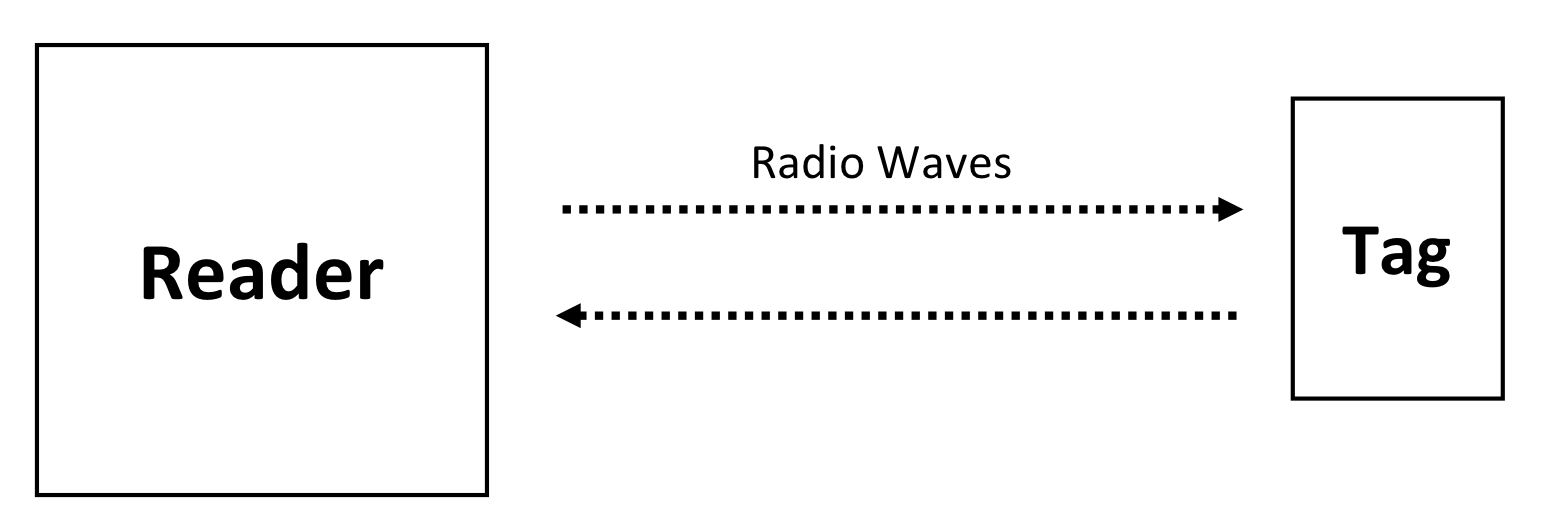
\includegraphics[width = 13cm]{Pictures/readertag}
	\caption{Reader Tag}
	\label{reader_tag}
\end{figure}
\subsubsection{RFID System}
Regarding the tags as shown in fig.\ref{rfid_system}, it can be either
\begin{itemize}
	\item Active tag which has its own power supply 
	\item Passive tag which relies on the radio waves as its source of energy that come from the reader 
	\item Semi-passive tag which has power supply, but for transmitting the feedback, it relies on the signal coming from reader
\end{itemize}
\begin{figure}[!htbp]
	\centering
	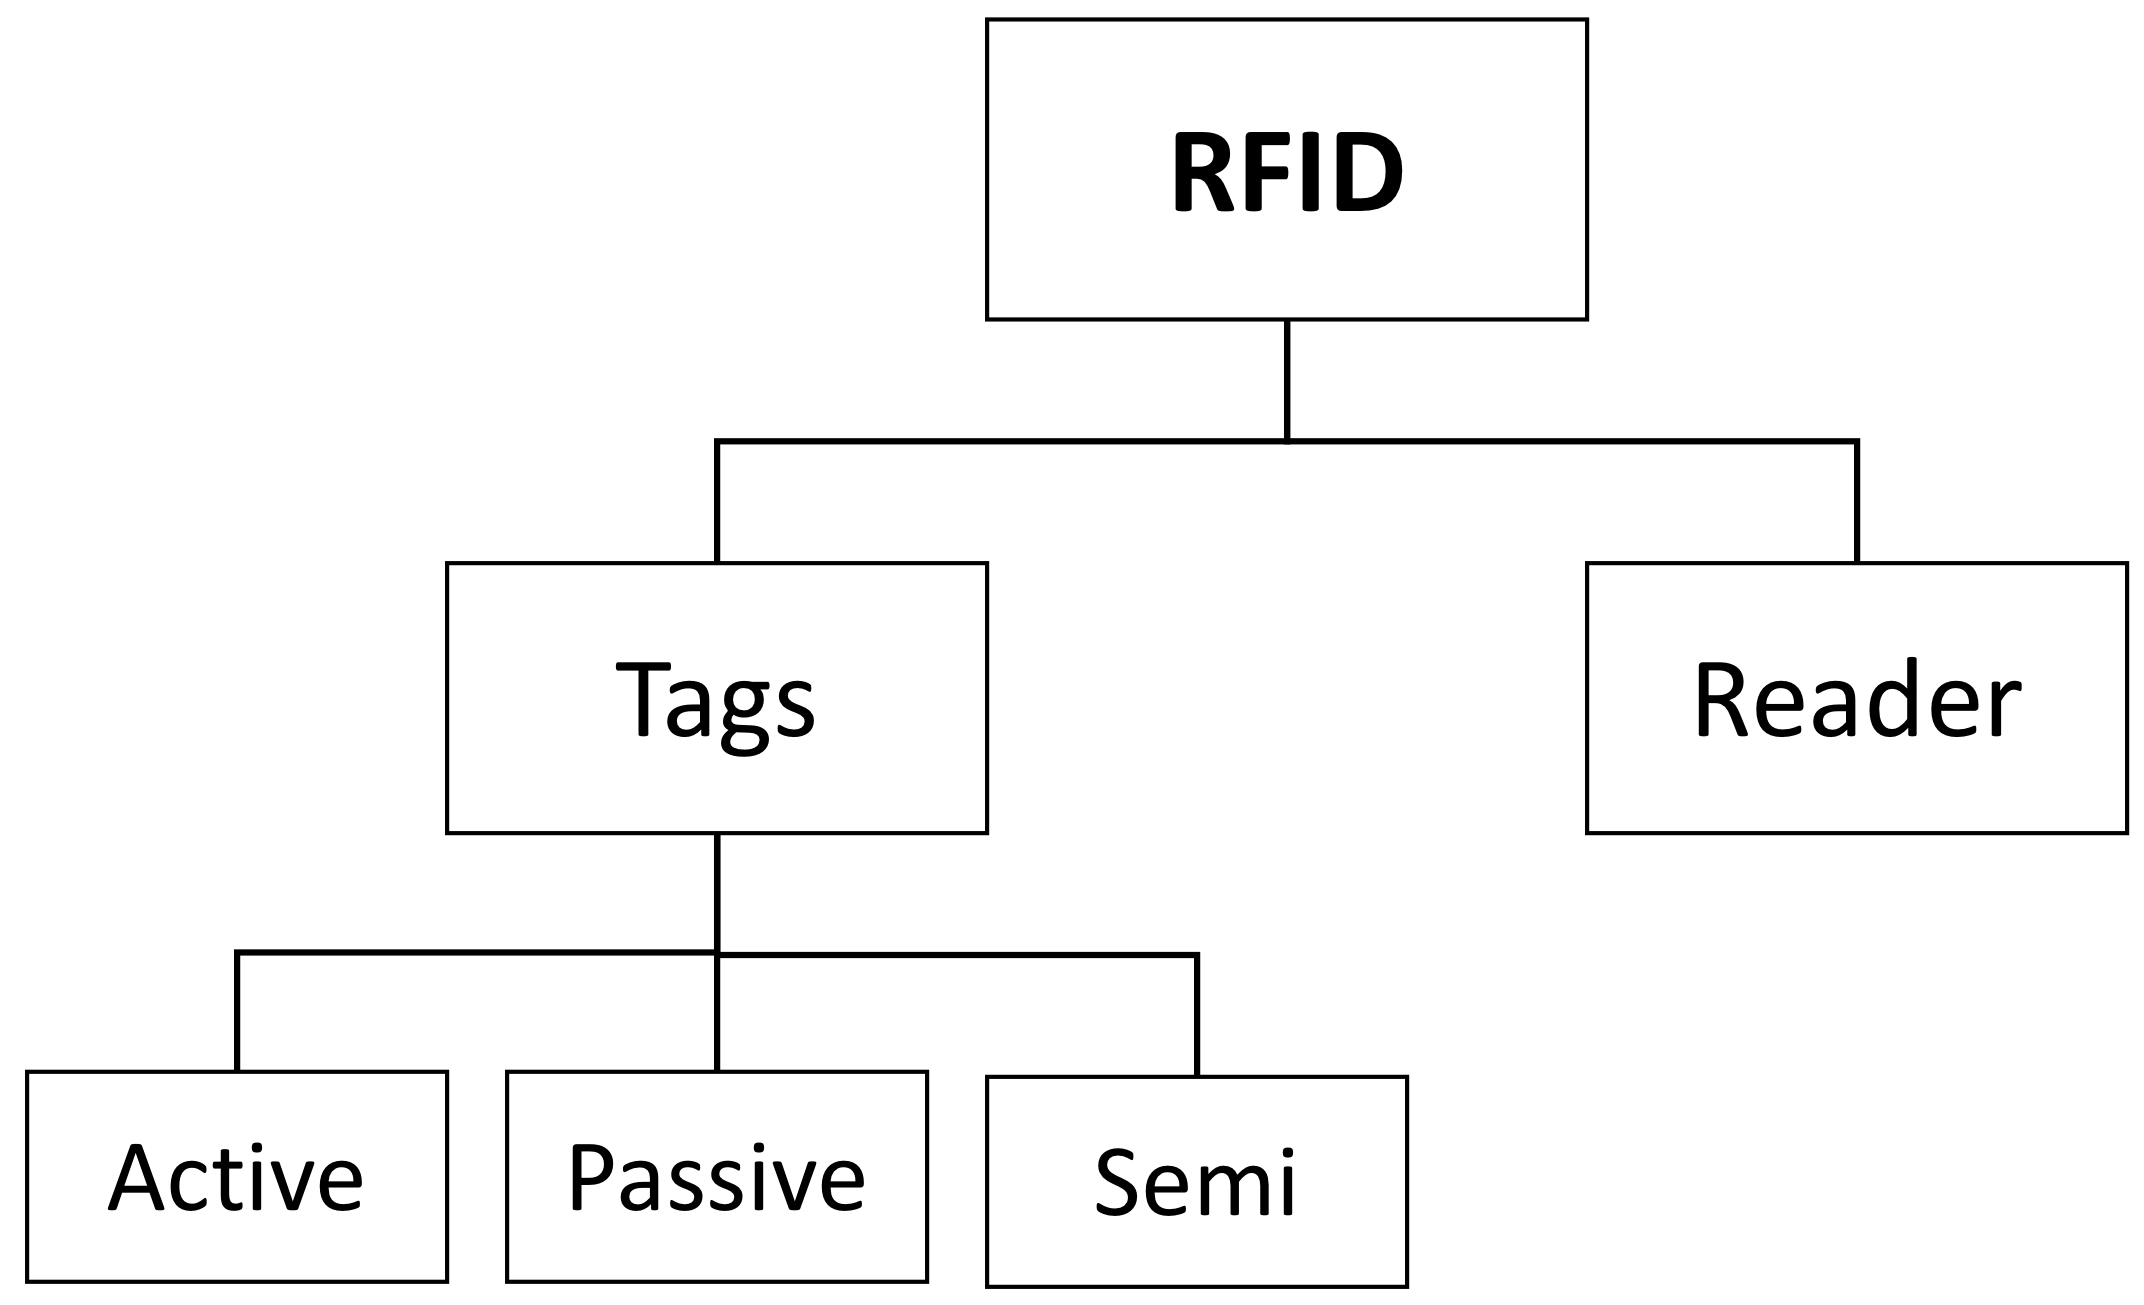
\includegraphics[width = 10cm]{Pictures/rfidsystem}
	\caption{RFID System}
	\label{rfid_system}
\end{figure}

\subsubsection{Working Principle}

The RFID consists of three main parts:
\begin{itemize}
		\item A Generator which generates the radio waves
		\item A signal detector which receives the feedback from the tag
		\item Micro-controller which processes the information from the generator and the detector\\
		\\
	\end{itemize}
The tags consists of:
\begin{itemize}
	\item Transponder: that receives radio waves and sends the feedback
	\item Rectifier Circuit: which stores the energy coming from the wave across the capacitor, and this energy is used as a power supply for the controller as well as the memory
\end{itemize}

\begin{figure}[!htbp]
	\centering
	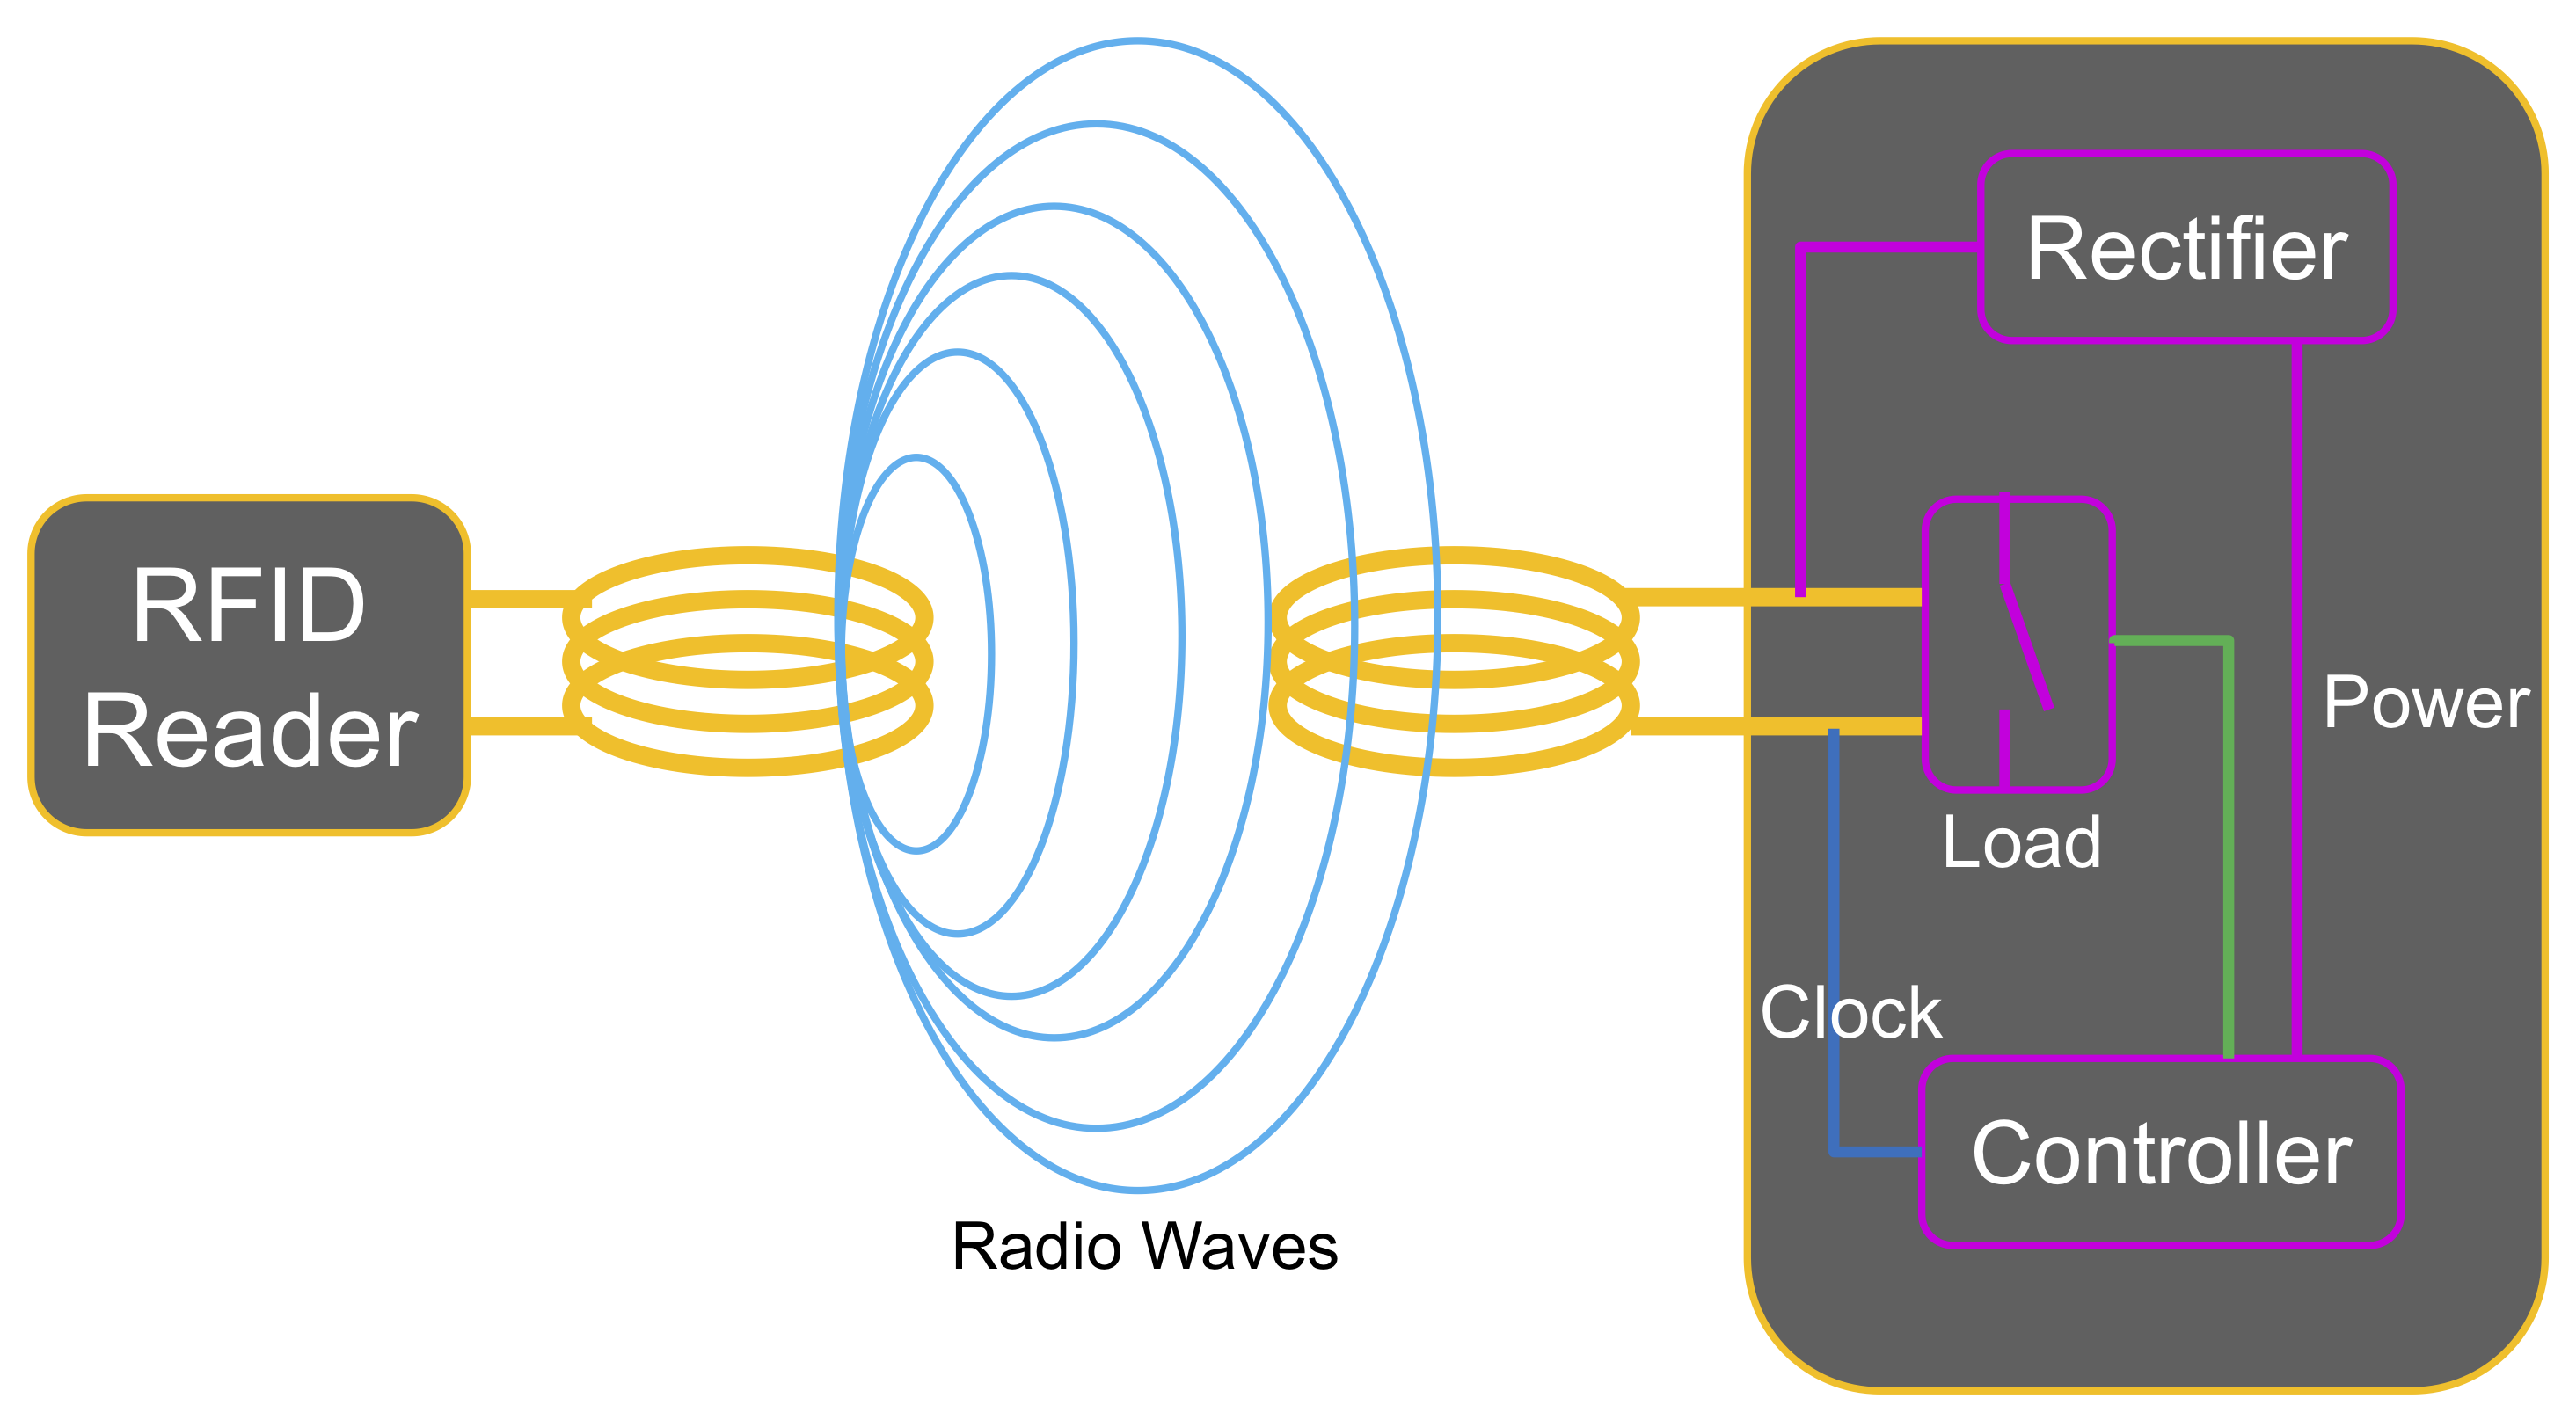
\includegraphics[width = 13cm]{Pictures/rfidtotag}
	\caption{Inductive Coupling}
	\label{rfid_to_tag}
\end{figure}
The whole process of sending the information between the tag and the reader is based on principle of "Inductive coupling" as shown in fig. \ref{rfid_to_tag}.
The reader is continuously sending radio waves with particular frequency. In this case, the reader and tag should be within the range of the frequency. The field which is generated by the reader is used coupling antenna of the tag, and due to the mutual coupling, the voltage is induced across the coil of the tag. The voltage is rectified and used as power supply for the controller and derive synchronization clock for the controller.\\
When the load circuit is connected to the coil, the current starts flowing through it. Therefore, when the load is switched on and off , the current will be turned on and off respectively leading to the induction of particular voltage in the reader. This method of switching the load is called load modulation. Thus, with the help of load modulation with respect to the data stored in the tag, the value of the induced voltage can be modified. Which leads to the generation of modulation on carrier frequency, thereby sending the data to the reader.\\

\subsection{Trilateration}
Trilateration is a method to compute the intersection point $P$ of three circles/spheres. For this, it is necessary to know the three center of the circles/spheres plus their corresponding radii. The basic idea to estimate the intersection point is to use the mathematical description of a sphere:
\begin{align}\label{Eq_Tri}
r^2 = (x-x_1)^2 + (y-y_1)^2 + (z-z_1)^2  
\end{align} 
where ($P_n=(x_n,y_n,z_n$)) is the center of the sphere \cite{Cotera.2016}. A few assumptions can be made to simplify (\ref{Eq_Tri}) for a flat floor/ 2D space. First of all, the z-component of all spheres can be neglected. Another assumption is that we define the origin of the first circle as the center of the coordinate system, the second along the x-axis with an distance (d) and the third shifted in x- (i) and y-direction (j), which is illustrated in following fig. \ref{Tri_1}.\\ 
\begin{figure}[!htbp]
 \centering
 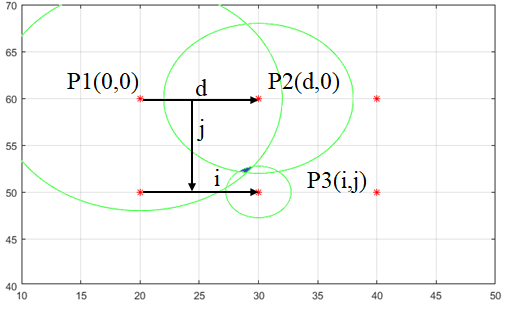
\includegraphics[width = 13cm]{Pictures/Trilateration_1}
 \caption{Overview Trilateration}
 \label{Tri_1}
 \end{figure}\\ 
With known positions of the center of the circles d, i and j can be computed in the following way\cite{Cotera.2016}:
\begin{align}
d = |P_2 - P_1| \\ 
e_x = \dfrac{1}{d}(P_2 - P_1) \\
a_x = P_3 - P_1 \\
i = e_x \cdot a_x \\
a_y = (P_3 - P_1) - i * e_x \\
e_y = \dfrac{a_y}{|a_y|} \\
j = e_y \cdot a_x
\end{align}
It has to be notice that $P_1$,$P_2$  and $P_3$ are 2D vectors, which represents the x- and y-coordinate of the points.\\ 
After obtaining these values, the relative distance from the origin of the coordinate system can be computed with the help of (\ref{Eq_Tri}) and the center of the circles $P_1$(0,0), $P_2$(0,d) and $P_3$(i,j) as follows:
\begin{align}
x_t = \dfrac{r_1^2 - r_2^2 + d^2}{2*d} \\
y_t = \dfrac{r_1^2 - r_3^2 + i^2 + j^2}{2*j} - i* \bigg(\dfrac{x_t}{j}\bigg) 
\end{align}
The absolute position of the intersection point is computed in following way:
\begin{align}
P = P_1 + e_x * x_t + e_y * y_t 
\end{align}
It can be seen, that those equations are using the first two points plus radii to estimate the x-coordinate and first and third point plus the estimated x-coordinate to estimate the y-coordinate.\\ 
